% Gambar alur autentikasi untuk README.
% Kompilasi: pdflatex alur-autentikasi.tex, lalu
% pdftoppm -png -r 200 -singlefile alur-autentikasi.pdf alur-autentikasi
\documentclass[tikz,border=14pt]{standalone}
\usepackage[scaled]{helvet}
\renewcommand{\familydefault}{\sfdefault}
\usepackage[T1]{fontenc}
\usetikzlibrary{arrows.meta,positioning,shapes.geometric,backgrounds,calc}

\definecolor{ink}{HTML}{0F172A}
\definecolor{subtle}{HTML}{64748B}
\definecolor{indigo}{HTML}{4338CA}
\definecolor{indigofill}{HTML}{EEF2FF}
\definecolor{okline}{HTML}{15803D}
\definecolor{okfill}{HTML}{F0FDF4}
\definecolor{badline}{HTML}{B91C1C}
\definecolor{badfill}{HTML}{FEF2F2}
\definecolor{cell}{HTML}{86EFAC}

\begin{document}
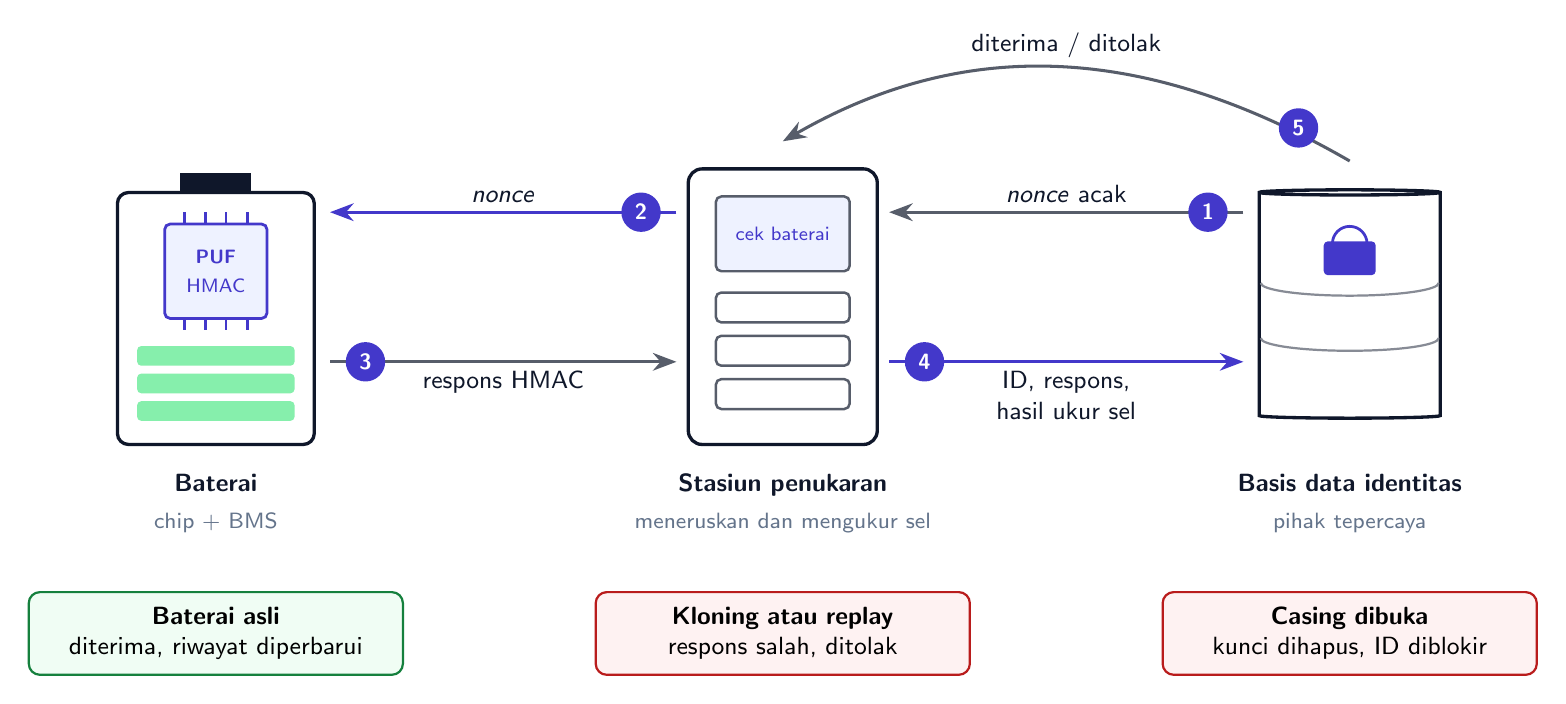
\begin{tikzpicture}[
  font=\sffamily,
  lbl/.style={font=\sffamily\small, text=ink, align=center},
  sub/.style={font=\sffamily\footnotesize, text=subtle, align=center},
  arrow/.style={-{Stealth[length=3mm]}, line width=1.1pt, draw=indigo},
  back/.style={-{Stealth[length=3mm]}, line width=1.1pt, draw=ink!70},
  num/.style={circle, fill=indigo, text=white, font=\sffamily\footnotesize\bfseries, inner sep=1.2pt, minimum size=5mm},
  msg/.style={font=\sffamily\small, text=ink, fill=white, inner sep=2pt},
  badge/.style={rounded corners=4pt, line width=0.8pt, font=\sffamily\small, align=center, minimum height=1.05cm, text width=4.4cm, inner sep=5pt}
]

% ---------- Baterai dengan chip ----------
\begin{scope}[shift={(0,0)}]
  \draw[ink, line width=1.2pt, rounded corners=4pt, fill=white] (-1.25,-1.6) rectangle (1.25,1.6);
  \fill[ink] (-0.45,1.6) rectangle (0.45,1.85);
  \foreach \y in {-1.3,-0.95,-0.6} \fill[cell, rounded corners=1.5pt] (-1.0,\y) rectangle (1.0,\y+0.25);
  % chip
  \draw[indigo, line width=1pt, fill=indigofill, rounded corners=2pt] (-0.65,0.0) rectangle (0.65,1.2);
  \foreach \x in {-0.4,-0.13,0.13,0.4} {
    \draw[indigo, line width=0.9pt] (\x,1.2) -- (\x,1.35);
    \draw[indigo, line width=0.9pt] (\x,0.0) -- (\x,-0.15);
  }
  \node[font=\sffamily\scriptsize\bfseries, text=indigo] at (0,0.78) {PUF};
  \node[font=\sffamily\scriptsize, text=indigo] at (0,0.42) {HMAC};
  \node[lbl, below=0.25cm] at (0,-1.6) {\textbf{Baterai}};
  \node[sub, below=0.75cm] at (0,-1.6) {chip + BMS};
\end{scope}

% ---------- Stasiun penukaran ----------
\begin{scope}[shift={(7.2,0)}]
  \draw[ink, line width=1.2pt, rounded corners=5pt, fill=white] (-1.2,-1.6) rectangle (1.2,1.9);
  \draw[ink!70, line width=0.9pt, rounded corners=2pt, fill=indigofill] (-0.85,0.6) rectangle (0.85,1.55);
  \node[font=\sffamily\scriptsize, text=indigo] at (0,1.07) {cek baterai};
  \foreach \y in {-0.05,-0.6,-1.15} \draw[ink!70, line width=0.9pt, rounded corners=2pt] (-0.85,\y) rectangle (0.85,\y+0.38);
  \node[lbl, below=0.25cm] at (0,-1.6) {\textbf{Stasiun penukaran}};
  \node[sub, below=0.75cm] at (0,-1.6) {meneruskan dan mengukur sel};
\end{scope}

% ---------- Basis data identitas ----------
\begin{scope}[shift={(14.4,0)}]
  \node[cylinder, shape border rotate=90, draw=ink, line width=1.2pt, fill=white,
        minimum width=2.3cm, minimum height=2.9cm, aspect=0.28] (db) at (0,0.15) {};
  \foreach \y in {0.45,-0.25} \draw[ink!50, line width=0.8pt] (-1.13,\y) arc[start angle=180, end angle=360, x radius=1.13, y radius=0.16];
  % gembok
  \draw[indigo, line width=1pt] (-0.22,0.95) arc[start angle=180, end angle=0, radius=0.22];
  \fill[indigo, rounded corners=1.5pt] (-0.33,0.55) rectangle (0.33,0.98);
  \node[lbl, below=0.25cm] at (0,-1.6) {\textbf{Basis data identitas}};
  \node[sub, below=0.75cm] at (0,-1.6) {pihak tepercaya};
\end{scope}

% ---------- Panah bernomor ----------
% 1: basis data -> stasiun (atas)
\draw[back] (13.05,1.35) -- (8.55,1.35) node[midway, msg, above=1pt] {\emph{nonce} acak};
\node[num] at (12.6,1.35) {1};
% 2: stasiun -> baterai (atas)
\draw[arrow] (5.85,1.35) -- (1.45,1.35) node[midway, msg, above=1pt] {\emph{nonce}};
\node[num] at (5.4,1.35) {2};
% 3: baterai -> stasiun (bawah)
\draw[back] (1.45,-0.55) -- (5.85,-0.55) node[midway, msg, below=1pt] {respons HMAC};
\node[num] at (1.9,-0.55) {3};
% 4: stasiun -> basis data (bawah)
\draw[arrow] (8.55,-0.55) -- (13.05,-0.55) node[midway, msg, below=1pt, align=center] {ID, respons,\\hasil ukur sel};
\node[num] at (9.0,-0.55) {4};
% 5: basis data -> stasiun (lengkung atas)
\draw[back] (14.4,2.0) to[out=150, in=30] node[midway, msg, above=1pt] {diterima / ditolak} (7.2,2.25);
\node[num] at (13.75,2.42) {5};

% ---------- Hasil ----------
\node[badge, draw=okline, fill=okfill] at (0,-4.0)
  {\textbf{Baterai asli}\\diterima, riwayat diperbarui};
\node[badge, draw=badline, fill=badfill] at (7.2,-4.0)
  {\textbf{Kloning atau \emph{replay}}\\respons salah, ditolak};
\node[badge, draw=badline, fill=badfill] at (14.4,-4.0)
  {\textbf{Casing dibuka}\\kunci dihapus, ID diblokir};

\end{tikzpicture}
\end{document}
